\section{Optimal Control of Pitch/Travel and Elevation with and without Feedback}\label{sec:prob4}
In this section we extend our model to include the remaining states: elevation, $e$, and elevation
rate, $\dot{e}$. We use a non-linear solver to compute an optimal trajectory in two dimensions,
and additionally constrain the elevation to avoid a restriction shaped as a bell-curve.

\subsection{State-space formulation}
The state-vector is extended with the remaining states, $x = \begin{bmatrix} \lambda & r & p & \dot{p} & e & \dot{e} \end{bmatrix}^T$, and the input-vector also contains the elevation setpoint fed to the internal controller, $u = \begin{bmatrix} p_c & e_c \end{bmatrix}^T$. The system is on the usual state-space form (\ref{eq:state_space_axbu}),
with
\begin{equation}
    \dot{x} =
    \underbrace{
    \begin{bmatrix}
    0 & 1 &      0     &      0     &      0     &      0    \\
    0 & 0 &    -K_2    &      0     &      0     &      0    \\
    0 & 0 &      0     &      1     &      0     &      0    \\
    0 & 0 & -K_1K_{pp} & -K_1K_{pd} &      0     &      0    \\
    0 & 0 &      0     &      0     &      0     &      1    \\
    0 & 0 &      0     &      0     & -K_3K_{ep} & -K_3K_{ed}
    \end{bmatrix}}_{A_c}
    x +
    \underbrace{
    \begin{bmatrix}
        0       &     0     \\
        0       &     0     \\
        0       &     0     \\
    K_1K_{pp}   &     0     \\
        0       &     0     \\
        0       & K_3K_{ep}
    \end{bmatrix}}_{B_c}
    u
    \label{eq:extended_state_space}
\end{equation}

\subsection{Discretization}
We discretize (\ref{eq:extended_state_space}) using the same method
as in section (\ref{sec:prob2}). That is, an approximation of the
discrete-time state-space matrices is
\begin{equation}
    A \approx I + hA_c
    \qquad\text{and}\qquad
    B \approx hB_c
\end{equation}
where $I$ is now the $6\times6$ identity matrix.

\subsection{Modelling the restriction}
A common application of optimal control is to implement restrictions,
such as avoiding physical objects, as constraints in the optimization
problem. Such restrictions can not be enforced when using only state-
feedback controllers.

We wish to restrict the helicopter head to move above a bell-shaped curve
\begin{equation}
    e_k \geq \alpha \exp (-\beta (\lambda_k - \lambda_t)^2 )
\end{equation}
for all timesteps $k$ over the solution horizon. Since this is a non-linear constraint, we can no longer use a QP solver. Instead, a non-linear solver is needed, and in this case, the MATLAB function fmincon was used with a SQP-type algorithm.

% \section{Notater for dagen: 16. mars} % Fikk fmincon til å fungere, med ikke-lineær constraint. % TODO: Test uten LQR. Lag egen slx hvor vi kopler ut LQR blokka.
% TODO: Kjør tuning tester. Juster Q_LQR.

\subsection{Objective function}
For this assignment, the cost function was the same as in equation (\ref{eq:trajectory_cost}), but with an extra term for penalizing elevation. We chose to set up the cost function on a more general form:
\begin{equation}
    \phi=\sum(x^{T}Q_{LQR}x+u^{T}R_{LQR}u)
\end{equation}
Here, $Q_{LQR}$ and $R{LQR}$ are diagonal matrices, with unity weight on $q_{travel}$, $r_{pitch}$ and $r_{elevation}$, so that it corresponds with the extended state and input vectors (\ref{eq:}). %vil her ha label på inlinefuncen lenger oppe.

%This formulation makes it possible to easily put some weight on the other states as well, if deviation in these states should be penalized.

\subsection{Results}

For controlling the helicopter, we ended on a horizon of $N=60$ timesteps, or 15 seconds. This gave us an optimal trajectory that looked much the same as for assignment 3 for pitch and travel. In addition, an elevator trajectory just touching the top of the bell curve constraint was also calculated. The suggested horizon of $N=40$ did not terminate in reasonable time, and was therefore replaced by a longer horizon giving reasonable results.%forslag til bedre formulering?

The solution without feedback acted in the same manner as it did in section (\ref{sec:prob2}). As can be seen in figure (??) !!!!!, the real trajectory of travel and elevation tried to follow the optimal solution, but the effect of not having a perfect model becomes more and more clear as time passes, and at the end of the horizon, the travel drifted away from the solution just like in section (\ref{sec:prob2}).

Using state feedback LQR, the helicopter managed to follow the calculated trajectory quite good after some tuning. As in section (\ref{sec:prob3}), it was appropriate to weight deviation(s) in travel (and here also elevation) more than deviation in pitch. When the regulator is working on an inaccurate model, it is for the task given more constructive to try to follow the travel and elevation trajectories rather than the ideal, linearized input trajectory. This input will, given the unlinearities of the model, not lead to an appropriate response for the trajectories. The result, with different weights on the states of $Q_{LQR}$ can be seen in the following figures. %legge inn typ 3 figurer her med den beste og 2-3dårligere responser og i tillegg skrive på hva de ulike vektene er.

One thing worth noticing is that the trajectory of elevation consequently falls below the constraint at the peak of the constraint. We believe this is due to the fact that our model suggests that there is no link between the model for elevation, and that of pitch. They are in fact linked, and because of this, the regulator doesn't manage to meet both demands perfectly at the same time, and we get a deviation. If the model would include this crossing terms, the result would probably be better. The problem with this approach is that it leads to a non linear objective function, which takes longer time to compute for the solver.
% TODO: Add figure showing the helicopter following the non-linear constraint. Showing the associated input. Explain why the input looks like it does.
\begin{figure}[htb]
	\centering
   	 \makebox[\textwidth][c]{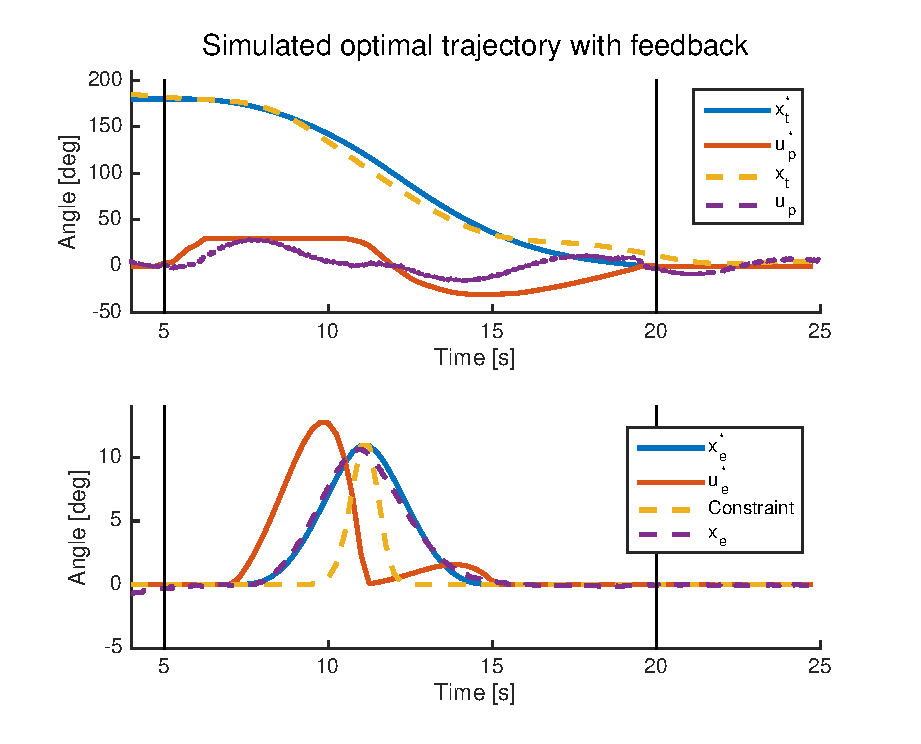
\includegraphics[width=1.2\textwidth]{figures/day4_cl/plot_day4_CL_q_20_1_1_1_30_10}}
	\caption{Plot day 4 closed loop Q=diag(20 1 1 1 30 10)}
	\label{fig:day4_cl_plot_20_1_1_1_30_10}
\end{figure}

% Notation:
% x_e^*: Computed elevation trajectory
% x_t^*: Computed travel trajectory
% u_p^*: Computed pitch setpoint sequence
% u_e^*: Computed elevation setpoint sequence


% Notat
% Cirka 11 sek ut i simuleringa, så ser vi at det er avvik mellom humpen og faktisk elevation, samtidig som det er avvik mellom travel-bane og faktisk travel. Vi har forsøkt å tune slik at elevation følger humpen tettere, men uten hell.

% Grunnen til dette tror vi er fordi det er en tradeoff i virkeligheten mellom å følge travel-banen og humpen. For å følge humpen bedre, så brukes pitch på en slik måte at det blir større avvik fra travel-banen. I modellen antas at pitch og elevation er fullstendig separerte, og dette problemet skal i teorien ikke oppstå. Men i virkeligheten er det en kobling.

% TODO: Forklar dette fenomenet. Referér til figuren, ved hump-toppen.
\begin{figure}[htb]
	\centering
   	 \makebox[\textwidth][c]{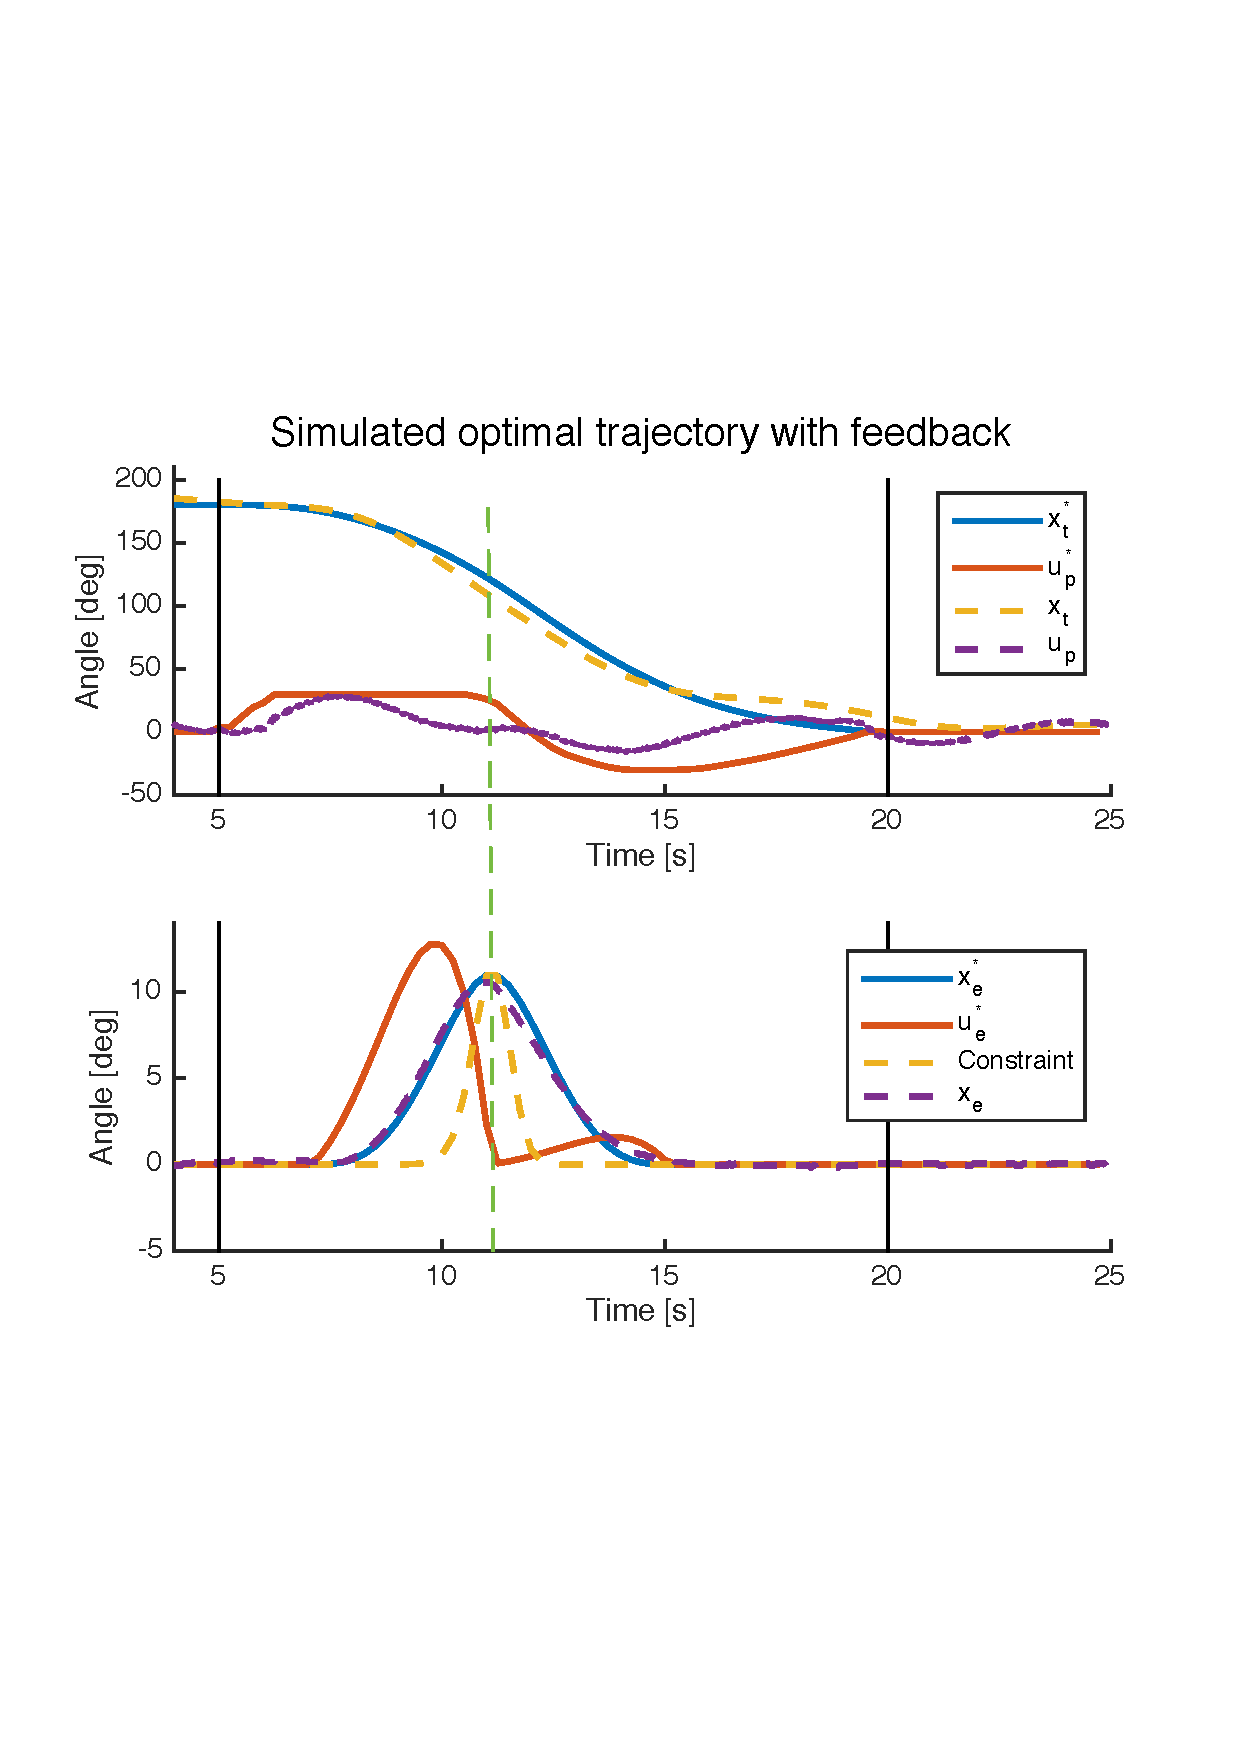
\includegraphics[width=1.2\textwidth]{figures/day4_cl/plot_day4_CL_q_20_1_1_1_20_1_marked2}}
	\caption{Coupling between pitch and elevation}
	\label{fig:coupling_pitch_elev}
\end{figure}
